\documentclass[conference]{IEEEtran}
\IEEEoverridecommandlockouts
% The preceding line is only needed to identify funding in the first footnote. If that is unneeded, please comment it out.

\usepackage{cite}
\usepackage{amsmath,amssymb,amsfonts}
\usepackage{algorithmic}
\usepackage{graphicx}
\usepackage{textcomp}
\usepackage{xcolor}
\usepackage{url}
\usepackage{tikz}
\usetikzlibrary{arrows.meta,fit,backgrounds}

\def\BibTeX{{\rm B\kern-.05em{\sc i\kern-.025em b}\kern-.08em
    T\kern-.1667em\lower.7ex\hbox{E}\kern-.125emX}}

\begin{document}

\title{CoProof: A Collaborative Platform for AI-Assisted Formal
Proof Development in Lean~4%
\thanks{[PLACEHOLDER: Identify applicable funding agency here. If none, delete this.]}
}

\author{
\IEEEauthorblockN{David Alejandro L\'opez Torres}
\IEEEauthorblockA{\textit{Software Development Engineering} \\
\textit{CETI Colomos}\\
Guadalajara, Mexico \\
a22310432@ceti.mx}
\and
\IEEEauthorblockN{Daniel Tejeda Saavedra}
\IEEEauthorblockA{\textit{Software Development Engineering} \\
\textit{CETI Colomos}\\
Guadalajara, Mexico \\
a22310431@ceti.mx}
\and
\IEEEauthorblockN{Emiliano Flores M\'arquez}
\IEEEauthorblockA{\textit{Software Development Engineering} \\
\textit{CETI Colomos}\\
Guadalajara, Mexico \\
a22110044@ceti.mx}
}

\maketitle

% -------------------------------------------------------------------------
\begin{abstract}
% PLACEHOLDER: Write a concise abstract (150--250 words).
% Do NOT use symbols, special characters, footnotes, or math here.
\textit{[PLACEHOLDER --- Abstract goes here.]}
\end{abstract}

\begin{IEEEkeywords}
formal verification, Lean~4, Mathlib, collaborative proof development,
distributed systems, \textit{[PLACEHOLDER --- add keywords]}
\end{IEEEkeywords}

% =========================================================================
\section{Introduction}
\label{sec:introduction}
% PLACEHOLDER: Motivate the problem, state contributions clearly, and
% outline the rest of the paper.
\textit{[PLACEHOLDER --- Introduction goes here.]}

% =========================================================================
\section{Related Work}
\label{sec:related}
% PLACEHOLDER: Survey related work on interactive theorem provers,
% collaborative verification platforms, and proof engineering toolchains.
\textit{[PLACEHOLDER --- Related Work goes here.]}

% =========================================================================
\section{Materials and Methods}
\label{sec:materials-methods}

% -------------------------------------------------------------------------
\subsection{Materials}
\label{subsec:materials}

CoProof was developed and deployed across two hardware tiers. The
development host was an x86-64 workstation running Windows~11; the
computation cluster comprised four Raspberry~Pi~4 Model~B units
(ARM Cortex-A72, 64-bit) connected over a private LAN
(\texttt{192.168.1.0/24}), provisioned with Rocky~Linux~10 (aarch64) and
managed through OpenHPC~\cite{ref:openhpc}, SLURM~\cite{ref:slurm} as
the workload scheduler, and OpenMPI~\cite{ref:openmpi} for distributed
execution. All platform services were containerized with Docker and
orchestrated via Docker~Compose.

The persistence layer used PostgreSQL~15 (Alpine) as the relational store
and Redis~7 (Alpine) as both the message broker and distributed cache.
The backend API was implemented in Python~3.11 (Debian Bookworm slim
container) with Flask~3.1.3, SQLAlchemy~2.0.47, and Flask-Migrate~4.1.0
(Alembic) for schema management; \texttt{psycopg2-binary}~2.9.11 served
as the PostgreSQL adapter. Authentication relied on JWT tokens issued
through Flask-JWT-Extended~4.7.1, with GitHub OAuth~2.0 (scopes:
\texttt{repo}, \texttt{read:user}, \texttt{user:email}) as the identity
provider.

Asynchronous task execution was handled by Celery~5.6.2 backed by
Redis~7.2.1, with three isolated queues: \texttt{lean\_queue},
\texttt{git\_engine\_queue}, and \texttt{computation\_queue}. Real-time
push notifications were delivered via Flask-SocketIO~5.6.1. Git
operations---repository cloning, atomic worktree transactions, and pull
request management---were issued programmatically using
GitPython~3.1.46 against the GitHub REST API~v3; theorem dependency
graphs were represented in-memory with NetworkX~3.6.1~\cite{ref:networkx}.
Production serving used \texttt{gunicorn}~25.1.0 with
\texttt{gevent}~25.9.1 workers. Request/response serialization was
handled by marshmallow~4.2.2. The frontend was built with
Angular~21.2.0 and TypeScript~5.9.2, bundled via
\texttt{@angular/cli}~21.2.0, using RxJS~7.8.0 for reactive HTTP
communication; Nginx served the compiled static assets inside the
frontend container.

The formal verification service ran in an isolated Ubuntu~22.04
container. Lean~4~\cite{ref:lean4} was installed and version-managed
through \texttt{elan}; the Lean toolchain version was pinned to the one
declared in Mathlib4~\cite{ref:mathlib4} at commit
\texttt{29dcec074de168ac2bf835a77ef68bbe069194c5}, which was compiled in
full via \texttt{lake exe cache get \&\& lake build}. The compiled
\texttt{LEAN\_PATH} exposed seven Mathlib4 sub-packages: \texttt{Qq},
\texttt{aesop}, \texttt{Cli}, \texttt{importGraph},
\texttt{LeanSearchClient}, \texttt{batteries}, and
\texttt{proofwidgets}. The service accepted proof snippets over a Celery
task interface (\texttt{lean\_queue}) and invoked the Lean~4 executable
on temporary files, parsing compiler output to extract theorem names,
line positions, error messages, and return codes.

Verification correctness was evaluated on a 100-theorem benchmark derived
from LeanDojo~\cite{ref:leandojo}, sourcing raw \texttt{.lean} files from
the public Mathlib4 GitHub repository at their respective commits.
Benchmark analysis used \texttt{matplotlib} and \texttt{numpy}. The test
suite across all Python services used \texttt{pytest}~9.0.2,
\texttt{pytest-flask}~1.3.0, and \texttt{pytest-mock}; code quality was
enforced with \texttt{black} and \texttt{flake8}.

Fig.~\ref{fig:system-overview} illustrates the complete system
architecture across hardware tiers and containerized services.

\begin{figure*}[htbp]
\centering
\resizebox{\linewidth}{!}{%
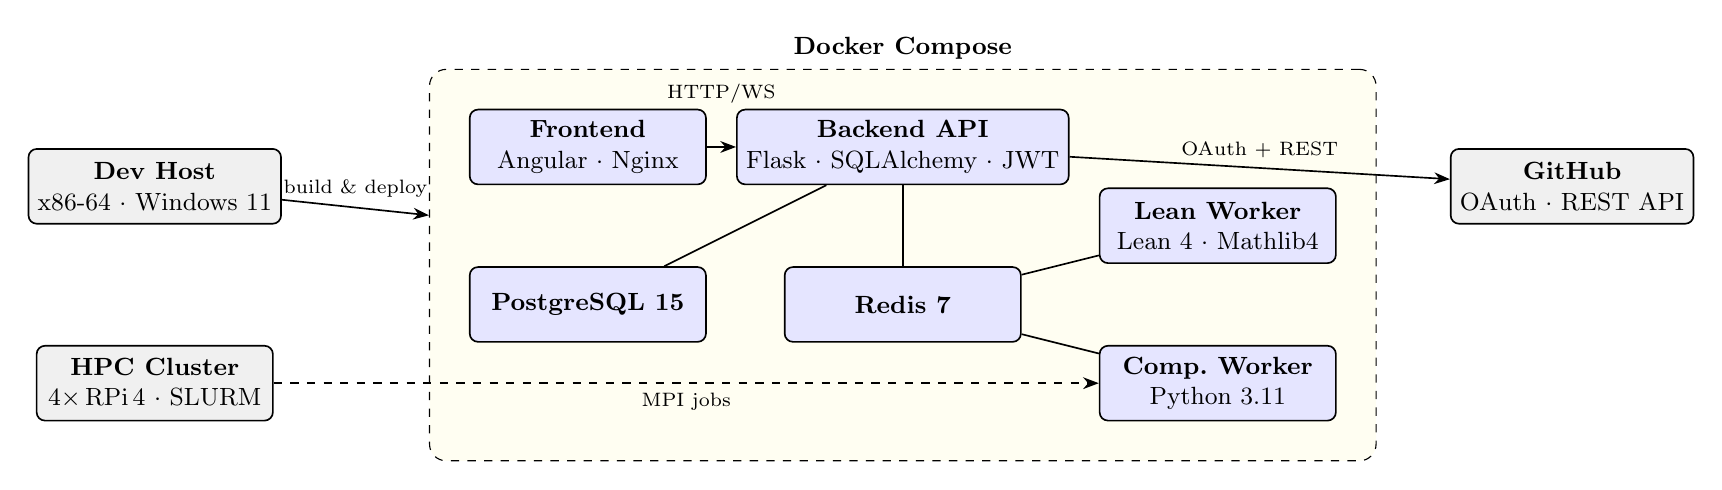
\begin{tikzpicture}[
  box/.style={draw, rounded corners=3pt, fill=blue!10,
              minimum width=3cm, minimum height=0.95cm, align=center, font=\small},
  ext/.style={draw, rounded corners=3pt, fill=gray!12,
              minimum width=3cm, minimum height=0.95cm, align=center, font=\small},
  >=Stealth, semithick
]
  % Internal (Docker) nodes
  \node[box] (fe)  at (2,   2)  {\textbf{Frontend}\\Angular $\cdot$ Nginx};
  \node[box] (api) at (6,   2)  {\textbf{Backend API}\\Flask $\cdot$ SQLAlchemy $\cdot$ JWT};
  \node[box] (pg)  at (2,   0)  {\textbf{PostgreSQL~15}};
  \node[box] (rd)  at (6,   0)  {\textbf{Redis~7}};
  \node[box] (lw)  at (10,  1)  {\textbf{Lean Worker}\\Lean~4 $\cdot$ Mathlib4};
  \node[box] (cw)  at (10, -1)  {\textbf{Comp.\ Worker}\\Python 3.11};
  % Docker Compose bounding box (drawn behind nodes)
  \begin{scope}[on background layer]
    \node[draw, dashed, rounded corners=6pt, fill=yellow!5, inner sep=0.5cm,
          fit=(fe)(api)(pg)(rd)(lw)(cw),
          label={[font=\small\bfseries]above:Docker Compose}] (docker) {};
  \end{scope}
  % External nodes
  \node[ext] (dev)     at (-3.5,  1.5) {\textbf{Dev Host}\\x86-64 $\cdot$ Windows~11};
  \node[ext] (cluster) at (-3.5, -1.0) {\textbf{HPC Cluster}\\4$\times$\,RPi\,4 $\cdot$ SLURM};
  \node[ext] (gh)      at (14.5,  1.5) {\textbf{GitHub}\\OAuth $\cdot$ REST API};
  % Connections
  \draw[->]        (dev)     -- (docker) node[midway, above, font=\scriptsize] {build \& deploy};
  \draw[->, dashed](cluster) -- (cw)     node[midway, below, font=\scriptsize] {MPI jobs};
  \draw[->]        (fe)      -- (api)    node[midway, above, yshift=12pt, font=\scriptsize] {HTTP/WS};
  \draw            (api)     -- (pg);
  \draw            (api)     -- (rd);
  \draw            (rd)      -- (lw);
  \draw            (rd)      -- (cw);
  \draw[->]        (api)     -- (gh)     node[midway, above, font=\scriptsize] {OAuth + REST};
\end{tikzpicture}%
}
\caption{CoProof system overview: hardware tiers and containerized services.}
\label{fig:system-overview}
\end{figure*}

% -------------------------------------------------------------------------
\subsection{Methods}
\label{subsec:methods}

\subsubsection{Development Methodology}
\label{subsubsec:dev-methodology}

CoProof was developed by a three-person team using a hybrid methodology:
a phase-gated discipline for the backend followed by Scrum-style sprints
for frontend integration. The process began with a full specification
layer---user stories with testable acceptance criteria, HTML wireframes
for every principal view, and architecture documents with UML class
diagrams per service---before any implementation began.

The backend was then built across six sequential phases, each with an
explicit exit condition: (1)~infrastructure and application factory,
(2)~database schema and ORM models, (3)~stateless Git engine with
distributed locking, (4)~domain service layer, (5)~RESTful API, and
(6)~asynchronous task workers. Only once all six phases were stable did
the team switch to three one-week sprints covering frontend views, the
natural-language-to-Lean translation flow, and AI-assisted suggestions,
followed by a hard feature freeze and a dedicated testing week.

Quality was maintained continuously through three mechanisms applied
across all stages. A GitHub Actions CI pipeline executed the full Docker
build, the \texttt{pytest} integration suite, and the Angular Vitest unit
suite on every pull request, blocking any merge on failure. A
zero-defects rule---adapted from Spolsky's
formulation~\cite{ref:spolsky}---required all high-priority bugs to be
closed before new feature work began, enforced at each sprint kickoff.
Every change additionally required peer code review against a mandatory
checklist. Two structured usability sessions with external participants
were conducted during the final testing week, with each friction point
logged as a GitHub Issue and resolved before delivery.

Fig.~\ref{fig:dev-process} summarizes the three-stage development process
and the continuous quality mechanisms.

\begin{figure*}[htbp]
\centering
\resizebox{\linewidth}{!}{%
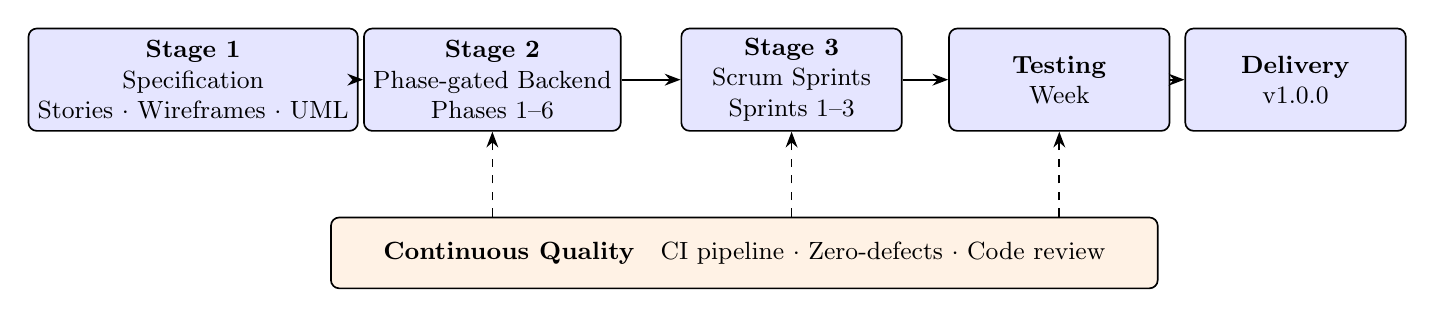
\begin{tikzpicture}[
  stage/.style={draw, rounded corners=3pt, fill=blue!10,
                minimum width=2.8cm, minimum height=1.3cm, align=center, font=\small},
  qa/.style={draw, rounded corners=3pt, fill=orange!10,
             minimum width=10.5cm, minimum height=0.9cm, align=center, font=\small},
  >=Stealth, semithick
]
  \node[stage] (s1) at (0,    0) {\textbf{Stage~1}\\Specification\\Stories $\cdot$ Wireframes $\cdot$ UML};
  \node[stage] (s2) at (3.8,  0) {\textbf{Stage~2}\\Phase-gated Backend\\Phases~1--6};
  \node[stage] (s3) at (7.6,  0) {\textbf{Stage~3}\\Scrum Sprints\\Sprints~1--3};
  \node[stage] (s4) at (11.0, 0) {\textbf{Testing}\\Week};
  \node[stage] (s5) at (14.0, 0) {\textbf{Delivery}\\v1.0.0};
  \node[qa]    (qa) at (7.0, -2.2) {\textbf{Continuous Quality}\quad CI pipeline $\cdot$ Zero-defects $\cdot$ Code review};
  \draw[->] (s1) -- (s2);
  \draw[->] (s2) -- (s3);
  \draw[->] (s3) -- (s4);
  \draw[->] (s4) -- (s5);
  \draw[->, dashed] (qa.north -| s2.south) -- (s2.south);
  \draw[->, dashed] (qa.north -| s3.south) -- (s3.south);
  \draw[->, dashed] (qa.north -| s4.south) -- (s4.south);
\end{tikzpicture}%
}
\caption{CoProof development process overview.}
\label{fig:dev-process}
\end{figure*}

\subsubsection{Execution Methodology}
\label{subsubsec:exec-methodology}

At runtime, CoProof organises every user action around a \emph{proof
graph}: a directed acyclic graph~(DAG) where each node maps one-to-one
to a \texttt{.lean} file in a GitHub repository. A project begins when
an authenticated user submits a goal statement; the backend pre-compiles
that goal through the Lean verification service before creating the
GitHub repository, then pushes three seed files---\texttt{Definitions.lean},
\texttt{root/main.lean}, and \texttt{root/main.tex}---and records a root
node in \texttt{sorry} state in PostgreSQL.

From that point, the user decomposes the proof by submitting \emph{node
splits}: Lean snippets that replace a \texttt{sorry} with a structured
proof referencing new child lemmas. Each split is verified synchronously
by the Lean worker before reaching GitHub; only a passing compilation
triggers the creation of a feature branch and a pull request. Merging
the PR fires a push webhook that reindexes the repository and creates
the corresponding child nodes in the database, each inheriting
\texttt{sorry} state. Leaf nodes are closed by submitting a complete
proof via the solve endpoint, which follows the same verify-branch-PR
cycle; validated states then propagate upward through the graph until
the root is fully proven.

For sub-goals that require empirical or numerical evidence rather than a
symbolic proof, the platform supports \emph{computation nodes}. A
computation node is created as a child of a proof node: the backend
extracts the parent theorem's Lean signature, generates a child
\texttt{.lean} stub using a typed axiom as placeholder, injects the
axiom's import into the parent, verifies the combined files with Lean,
and opens a PR with the new artifacts. The user then submits Python
source code through the compute endpoint; the computation worker
executes it in a sandboxed subprocess and returns a structured result
with an evidence value and a \texttt{sufficient} boolean. If evidence
is sufficient, the backend replaces the axiom with a concrete Lean
definition embedding the evidence, re-verifies through the Lean worker,
and opens a final PR. All write operations---splits, solves, and
computations---are protected by Redis-based distributed locks that
prevent concurrent modifications to the same repository.

Fig.~\ref{fig:exec-flow} depicts the complete proof execution pipeline,
including project creation, node-split, node-solve, computation node,
and collaboration/locking flows.

\begin{figure*}[htbp]
\centering
\resizebox{\linewidth}{!}{%
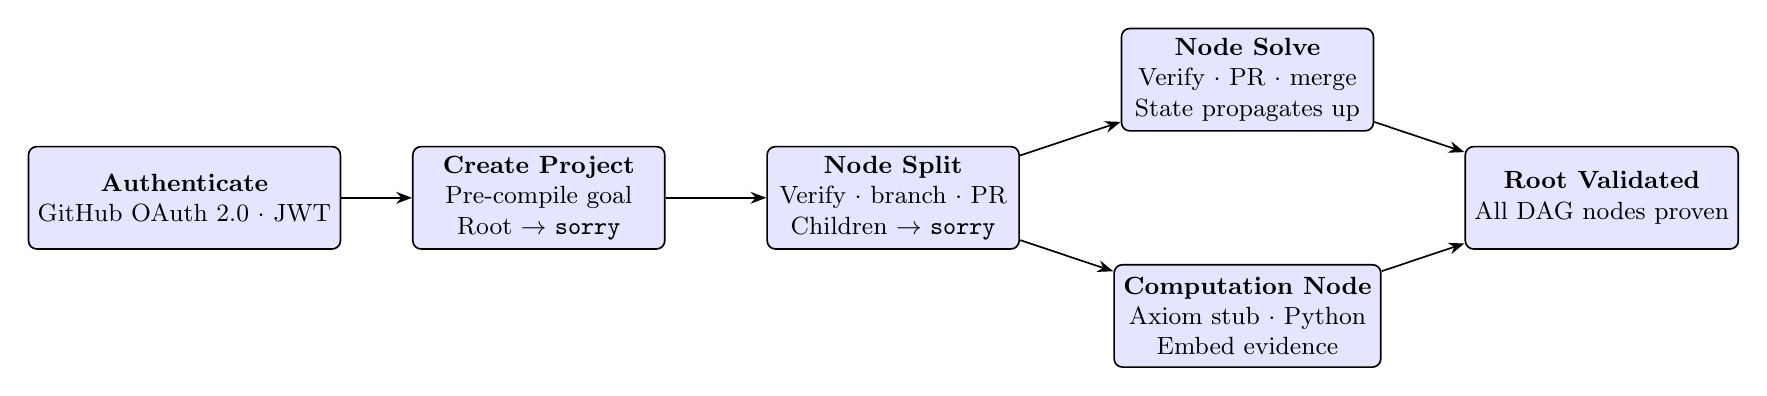
\begin{tikzpicture}[
  box/.style={draw, rounded corners=3pt, fill=blue!10,
              minimum width=3.2cm, minimum height=1.3cm, align=center, font=\small},
  >=Stealth, semithick
]
  \node[box] (auth)    at (0,     0)   {\textbf{Authenticate}\\GitHub OAuth~2.0 $\cdot$ JWT};
  \node[box] (create)  at (4.5,   0)   {\textbf{Create Project}\\Pre-compile goal\\Root $\to$ \texttt{sorry}};
  \node[box] (split)   at (9,     0)   {\textbf{Node Split}\\Verify $\cdot$ branch $\cdot$ PR\\Children $\to$ \texttt{sorry}};
  \node[box] (solve)   at (13.5,  1.5) {\textbf{Node Solve}\\Verify $\cdot$ PR $\cdot$ merge\\State propagates up};
  \node[box] (compute) at (13.5, -1.5) {\textbf{Computation Node}\\Axiom stub $\cdot$ Python\\Embed evidence};
  \node[box] (done)    at (18,    0)   {\textbf{Root Validated}\\All DAG nodes proven};
  \draw[->] (auth)    -- (create);
  \draw[->] (create)  -- (split);
  \draw[->] (split)   -- (solve);
  \draw[->] (split)   -- (compute);
  \draw[->] (solve)   -- (done);
  \draw[->] (compute) -- (done);
\end{tikzpicture}%
}
\caption{CoProof proof execution flow.}
\label{fig:exec-flow}
\end{figure*}

% =========================================================================
\section{Results}
\label{sec:results}

\subsection{Lean Verification Service}
\label{subsec:lean-benchmark}

A benchmark of 100 theorems drawn from the Mathlib4 library was executed
against the Lean verification service on November~27, 2025.
Table~\ref{tab:benchmark} summarises the outcome. All four failures were
caused by request timeouts (\texttt{api\_latency}~$= 35.0$\,s); no
failure was attributable to a Lean compilation error in the benchmark
inputs.

\begin{table}[htbp]
  \caption{Lean Verification Benchmark (100 Theorems)}
  \label{tab:benchmark}
  \centering
  \begin{tabular}{lr}
    \hline
    \textbf{Metric} & \textbf{Value} \\
    \hline
    Total submitted          & 100   \\
    With tactics / without   & 48 / 52 \\
    Successful verifications & 96    \\
    Failed (timeout)         & 4     \\
    Mock proofs used         & 0     \\
    Avg.\ fetch time (s)     & 1.02  \\
    Avg.\ API latency (s)    & 8.42  \\
    Avg.\ processing time (s)& 8.31  \\
    \hline
  \end{tabular}
\end{table}

\subsection{Implemented Services}
\label{subsec:services}

The platform was delivered as a nine-container Docker Compose stack.
Table~\ref{tab:services} lists every deployed service and its role.

\begin{table*}[htbp]
  \caption{Deployed Docker Compose Services}
  \label{tab:services}
  \centering
  \begin{tabular}{lll}
    \hline
    \textbf{Service} & \textbf{Technology} & \textbf{Role} \\
    \hline
    \texttt{web}                & Flask + SocketIO            & Backend API + real-time notifications \\
    \texttt{celery\_worker}     & Celery + Redis              & Git engine and general async tasks \\
    \texttt{lean-worker}        & Celery + Lean~4 (elan)      & Formal verification \\
    \texttt{nl2fl-worker}       & Celery + OpenRouter API     & Natural language $\to$ Lean translation \\
    \texttt{agents-worker}      & Celery + OpenRouter API     & LLM suggestion primitive \\
    \texttt{computation-worker} & Celery + Python subprocess  & Sandboxed numeric computation \\
    \texttt{frontend}           & Angular~21 + Nginx          & Single-page application \\
    \texttt{db}                 & PostgreSQL                  & Relational index and metadata \\
    \texttt{redis}              & Redis                       & Task queue broker + Redlock \\
    \hline
  \end{tabular}
\end{table*}

\subsection{Features Delivered}
\label{subsec:features}

All planned platform features were delivered at v1.0.0, as recorded in
Table~\ref{tab:features}.

\begin{table*}[htbp]
  \caption{Feature Delivery Status at v1.0.0}
  \label{tab:features}
  \centering
  \begin{tabular}{lc}
    \hline
    \textbf{Feature} & \textbf{Delivered} \\
    \hline
    GitHub OAuth~2.0 authentication (JWT pair) & $\checkmark$ \\
    Project creation with pre-compilation gate & $\checkmark$ \\
    DAG-based proof graph (root node, split, solve) & $\checkmark$ \\
    Lean verification worker (Ubuntu~22.04, Mathlib4 pinned) & $\checkmark$ \\
    Collaborative PR workflow via GitHub REST API & $\checkmark$ \\
    Webhook-triggered asynchronous reindexation & $\checkmark$ \\
    NL2FL translation pipeline (LLM + Lean feedback retry) & $\checkmark$ \\
    AI suggestion microservice (one-shot LLM prompt) & $\checkmark$ \\
    Computation nodes (Python sandbox + evidence embedding) & $\checkmark$ \\
    \LaTeX{} inline viewer in the frontend & $\checkmark$ \\
    Angular workspace view with DAG rendering & $\checkmark$ \\
    CI pipeline (GitHub Actions --- backend + frontend) & $\checkmark$ \\
    Per-user encrypted API key storage (AES-256-GCM) & $\checkmark$ \\
    \hline
  \end{tabular}
\end{table*}

\subsection{Continuous Integration Pipeline}
\label{subsec:ci}

The CI pipeline executed two parallel jobs on every push to \texttt{main}
or \texttt{develop} and on every pull request: a backend job
(\texttt{docker compose build} $\to$ \texttt{pytest} against a live
PostgreSQL instance $\to$ \texttt{docker compose down -v}) and a frontend
job (\texttt{npm ci} $\to$ \texttt{ng test} with Vitest $\to$ production
build). Average run time observed was under 5~minutes from push to result.

\subsection{Joel Test Self-Assessment}
\label{subsec:joel}

Each of the 12 Joel Test criteria~\cite{ref:spolsky} was evaluated against
documented artefacts at delivery (April~2026). All 12 criteria were met,
as recorded in Table~\ref{tab:joel}.

\begin{table}[htbp]
  \caption{Joel Test Results (April~2026)}
  \label{tab:joel}
  \centering
  \begin{tabular}{clc}
    \hline
    \textbf{\#} & \textbf{Criterion} & \textbf{Met} \\
    \hline
    1  & Source control              & $\checkmark$ \\
    2  & One-step build              & $\checkmark$ \\
    3  & Daily builds (CI)           & $\checkmark$ \\
    4  & Bug database                & $\checkmark$ \\
    5  & Fix bugs before new code    & $\checkmark$ \\
    6  & Up-to-date schedule         & $\checkmark$ \\
    7  & Spec before code            & $\checkmark$ \\
    8  & Quiet working conditions    & $\checkmark$ \\
    9  & Best tools available        & $\checkmark$ \\
    10 & Testers                     & $\checkmark$ \\
    11 & Coding interviews           & $\checkmark$ \\
    12 & Hallway usability testing   & $\checkmark$ \\
    \hline
  \end{tabular}
\end{table}

% =========================================================================
\section{Discussion}
\label{sec:discussion}

\subsection{Lean Verification Performance}
\label{subsec:disc-lean}

The 96\,\% success rate on the Mathlib4 benchmark confirms that the Lean
worker is operationally sound for the expected workload. All four failures
shared the same root cause: API latency exceeding the 35-second timeout
threshold, not a correctness defect in the verification logic. The average
processing time of 8.3\,s per theorem is consistent with Lean~4 compilation
times for medium-complexity theorems against a pre-compiled Mathlib4
environment. The absence of any mock proofs ensures that the numbers reflect
real verification against actual Lean source.

The timeout failures highlight a structural tension: theorems with long
tactic chains can exceed the wall-clock budget acceptable for a synchronous
API response. The current architecture mitigates this by placing Lean tasks
in a Celery queue with frontend polling, but the 45-second client timeout
still acts as a hard ceiling. For the project's current scope---short,
targeted leaf-node proofs---this ceiling is adequate; it becomes a
limitation for goals drawn from deeper layers of Mathlib.

\subsection{Architecture: Git as Source of Truth}
\label{subsec:disc-git}

Using GitHub as the authoritative content store and PostgreSQL as a fast
relational index is the most consequential architectural decision in the
system. It provides a collaborative PR-based workflow without building a
custom version control system and ensures that Lean source remains
auditable, fork-able, and independent of the platform's database. The
tradeoff is operational complexity: every write operation must execute a
multi-step Git transaction protected by a Redis Redlock to prevent
concurrent corruption.

In practice, transaction latency is acceptable for the expected concurrency
of an academic collaboration tool. The LRU \texttt{RepoPool} cache of bare
clones reduces redundant GitHub API calls significantly. At higher
concurrency levels, however, the Redlock becomes a serialisation bottleneck
per project; future optimisation would route read operations exclusively
through the PostgreSQL index.

\subsection{NL2FL Pipeline and LLM Integration}
\label{subsec:disc-nl2fl}

The natural-language-to-Lean pipeline introduces a non-deterministic element
into an otherwise deterministic verification chain. The retry loop that feeds
Lean error messages back to the LLM as context improves translation quality
but does not guarantee convergence. Empirically, output quality depends
heavily on the LLM's prior exposure to Lean~4 syntax and Mathlib idioms.
The decision to store per-user API keys encrypted (AES-256-GCM) rather than
using a shared platform key eliminates the platform's liability for usage
costs at the cost of additional friction for first-time users.

\subsection{Computation Nodes}
\label{subsec:disc-compute}

The computation node feature introduces a hybrid formal/empirical proof
model: a Python program produces numerical evidence that is embedded as a
concrete Lean definition replacing an axiom placeholder. This is a
non-standard use of Lean's type system---the ``proof'' of the axiom is a
datum, not a derivation---and its soundness depends entirely on the
correctness of the Python computation. The platform does not verify that the
embedded evidence value is consistent with the axiomatic claim it replaces;
that responsibility rests with the user. This feature is architecturally
separated from the verification path to make this distinction explicit, and
is most appropriate for theorems with a computable witness.

\subsection{Development Process}
\label{subsec:disc-process}

The spec-first, phase-gated approach produced a backend that was internally
consistent and largely defect-free before frontend integration began.
Committing architecture documents before implementation forced early
resolution of interface contracts (API shapes, model schemas, service
boundaries) and reduced late-stage integration surprises. The Joel Test
served as a process audit tool rather than a nominal checklist: every
passing criterion has a concrete artefact to substantiate it.

The three-sprint frontend integration cadence was tight relative to scope.
Several features---\LaTeX{} viewer, computation node UI, AI suggestion
UX---required non-trivial Angular component work that compressed available
testing time. Future projects of similar scope would benefit from a longer
frontend integration phase or earlier parallelisation of backend and
frontend work.

\subsection{Limitations}
\label{subsec:disc-limits}

\begin{itemize}
  \item \textbf{Lean timeout ceiling (45\,s).} Complex Mathlib theorems may
    consistently exceed the per-task wall-clock budget with no automatic
    adjustment based on historical compile times.
  \item \textbf{Single-branch collaboration.} The Redlock prevents
    corruption but does not mediate concurrent intent on the same node;
    last write wins at the Git level.
  \item \textbf{Computation sandbox isolation.} The Python subprocess runs
    in the container's process space without network isolation, resource
    caps, or time limits beyond the Celery task timeout.
  \item \textbf{NL2FL non-determinism.} Identical natural-language inputs
    may produce different Lean outputs across calls; there is no
    translation cache.
  \item \textbf{GitHub dependency.} All write operations require live
    GitHub API access; an outage prevents any proof editing even when
    content is locally cached.
\end{itemize}

\subsection{Future Work}
\label{subsec:future}

High-value extensions, ordered by estimated impact, include: adaptive
per-node Lean timeouts informed by historical compile times; tactic-aware
LLM integration wired to the node's current proof state; optimistic locking
and a conflict-resolution UI for concurrent node edits; \texttt{nsjail} or
\texttt{gVisor} sandboxing for computation nodes; a persistent NL2FL
translation cache; a one-click export of validated projects as
self-contained Lean~4 packages; Slurm/MPI dispatch for large-scale numerical
computations on the HPC cluster; public project discovery with fork support;
additional formal verification backends (Coq, Isabelle/HOL, Agda); and
real-time collaborative state broadcasts via the existing SocketIO
infrastructure.

% =========================================================================
\section{Conclusion}
\label{sec:conclusion}
% PLACEHOLDER: Summarize main contributions and outline future work
% (multi-language proof support, improved NL-to-Lean translation, larger
% HPC cluster integration).
\textit{[PLACEHOLDER --- Conclusion goes here.]}

% =========================================================================
\section*{Acknowledgment}
% PLACEHOLDER: Acknowledge contributors, institutions, and funding sources.
\textit{[PLACEHOLDER --- Acknowledgment goes here.]}

% =========================================================================
\begin{thebibliography}{00}

% --- Core theorem-prover references ---
\bibitem{ref:lean4}
  L. de Moura and S. Ullrich, ``The Lean~4 Theorem Prover and Programming
  Language,'' in \textit{Proc. 28th Int. Conf. Automated Deduction
  (CADE-28)}, 2021, pp.~625--635.
  % PLACEHOLDER: Verify exact venue, pages, and DOI.

\bibitem{ref:mathlib4}
  The Mathlib Community, ``Mathlib4: The Lean~4 Mathematical Library,''
  \textit{GitHub Repository}, 2024. [Online]. Available:
  \url{https://github.com/leanprover-community/mathlib4}
  % PLACEHOLDER: Replace with a peer-reviewed citation if available.

\bibitem{ref:leandojo}
  K. Yang \textit{et al.}, ``LeanDojo: Theorem Proving with
  Retrieval-Augmented Language Models,'' in \textit{Advances in Neural
  Information Processing Systems (NeurIPS)}, vol.~36, 2023.
  % PLACEHOLDER: Verify pages and DOI.

% --- HPC infrastructure references ---
\bibitem{ref:openhpc}
  K. Squyres \textit{et al.}, ``OpenHPC: Community Building Blocks for
  HPC Systems,'' in \textit{Proc. SC Companion}, 2016.
  % PLACEHOLDER: Replace with the correct OpenHPC reference.

\bibitem{ref:slurm}
  A. B. Yoo, M. A. Jette, and M. Grondona, ``SLURM: Simple Linux Utility
  for Resource Management,'' in \textit{Proc. Workshop on Job Scheduling
  Strategies for Parallel Processing (JSSPP)}, 2003, pp.~44--60.

\bibitem{ref:openmpi}
  E. Gabriel \textit{et al.}, ``Open MPI: Goals, Concept, and Design of a
  Next Generation MPI Implementation,'' in \textit{Proc. 11th European
  PVM/MPI Users' Group Meeting}, 2004, pp.~97--104.

% --- Software library references ---
\bibitem{ref:networkx}
  A. A. Hagberg, D. A. Schult, and P. J. Swart, ``Exploring Network
  Structure, Dynamics, and Function using NetworkX,'' in \textit{Proc.
  7th Python in Science Conf.\ (SciPy2008)}, 2008, pp.~11--15.

% --- Software engineering process references ---
\bibitem{ref:spolsky}
  J. Spolsky, ``Painless Bug Tracking,'' \textit{Joel on Software},
  Nov.\ 2000. [Online]. Available:
  \url{https://www.joelonsoftware.com/2000/11/08/painless-bug-tracking/}
  % PLACEHOLDER: Consider replacing with a peer-reviewed source on
  % zero-defect policies or defect management in agile projects.

% PLACEHOLDER: Add further references as required, e.g.:
%   Flask, Celery, GitPython, Angular, Docker, JWT (RFC 7519),
%   related collaborative proof platforms, etc.

\end{thebibliography}

\end{document}
